%% chapter 4 dataset, network structure, experiment and result
\chapter{PT网站的具体实现、改进与运营}
\label{cha:experiment}

在本章中, 将着重详细介绍前一章中提出的开发计划如何具体落地实施。同时, 在运营方面, 将介绍一些内测人员招募、培养用户习惯的实践经验。能够将自己的兴趣爱好推荐给他人, 并能使他人受益, 这样的课外实践令笔者收获了颇多心得。

\section{部署开发、运行、测试环境}

开发环境使用的是捷克Jetbrain公司的PhpStorm IDE(Integrated Development Environment, 集成开发环境)。它拥有完善的词头联想及代码补全功能, 能够极大地提高开发效率。

\begin{figure}[ht]
    \centering
    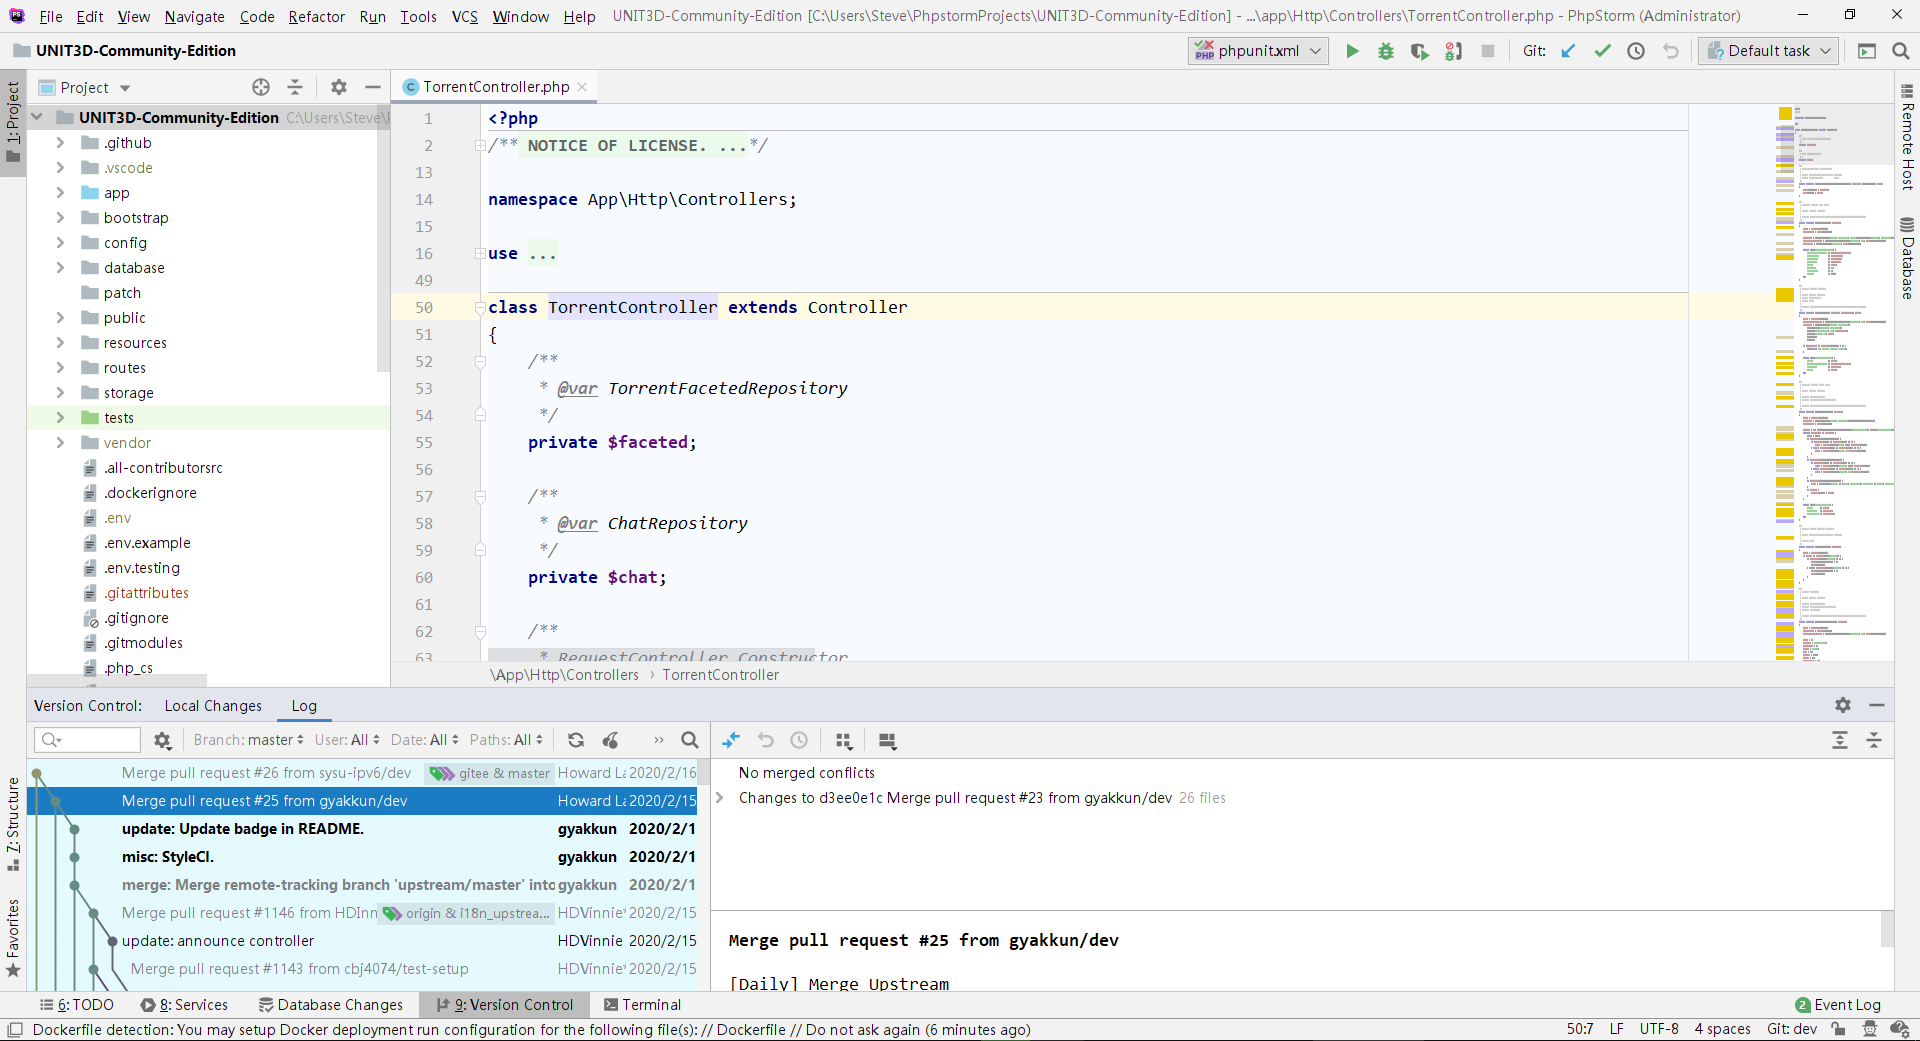
\includegraphics[width=0.8\textwidth]{support-files/4.1-phpstorm-ide.png}
    \caption{PhpStorm IDE}
    \label{fig:phpstormide}
\end{figure}

UNIT3D作者提供了一份手动部署的手册, 以及一个自动部署脚本, 但与当前各依赖包的最新版本有所脱节。为此, 笔者使用了站长howardlau同学提供的Dockerfile, 在每一次代码的修改、提交、推送之后, 交由代码托管方github的自动工作流系统\footnote{\url{https://help.github.com/en/github/collaborating-with-issues-and-pull-requests/github-flow}进行Docker\footnote{https://www.docker.com/}}镜像的构建与发布。若构建失败笔者将会收到邮件通知, 从而分载(Offload)了部分本应人工完成的编译时(Compile-time)测试工作。

\begin{figure}[ht]
    \centering
    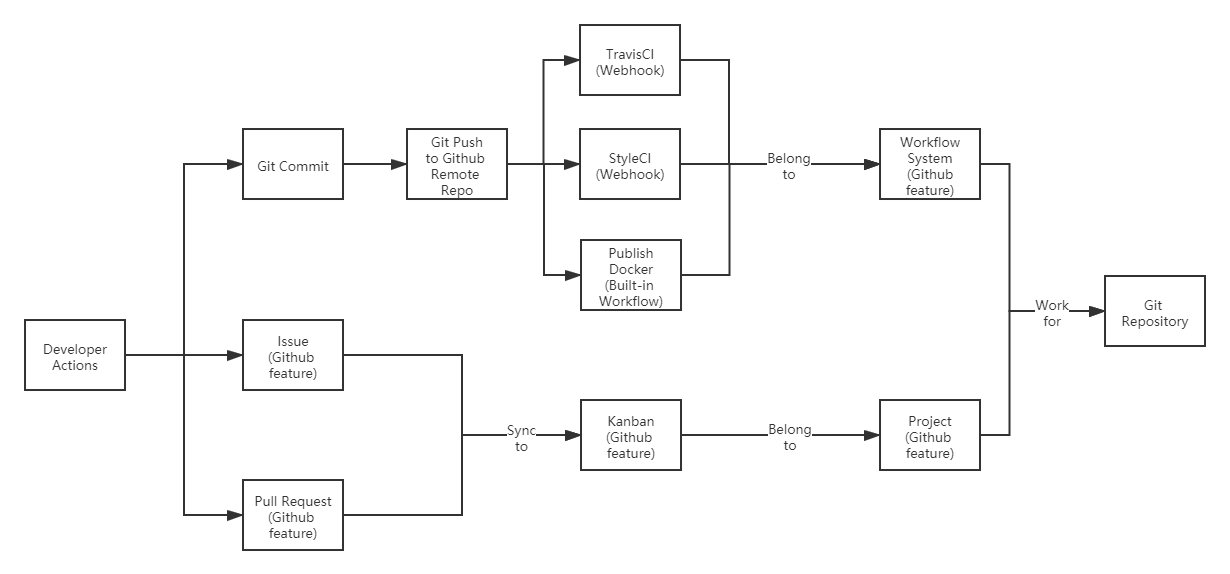
\includegraphics[width=\textwidth]{support-files/4.1-github-workflow.png}
    \caption{Github 工作流系统示意图}
    \label{fig:githubworkflow}
\end{figure}

% [图 (4.1-github-workflow) GITHUB 工作流 流程图]

除此之外, 笔者还使用了TravisCI\footnote{\url{https://travis-ci.org/}}进行部分用例测试, StyleCI\footnote{\url{https://styleci.io/}}来检查代码格式规范。两者都是各自领域优秀的持续集成(Continuos Integration, CI)测试工具, 基本上承担了大部分代码级别的测试工作, 效果见图 \ref{fig:ci}。具体的功能测试将在\ref{sec:preop}中的试运营部分给出描述。

\begin{figure}[h]
	\centering
    \begin{subfigure}{0.8\textwidth}
		\centering
		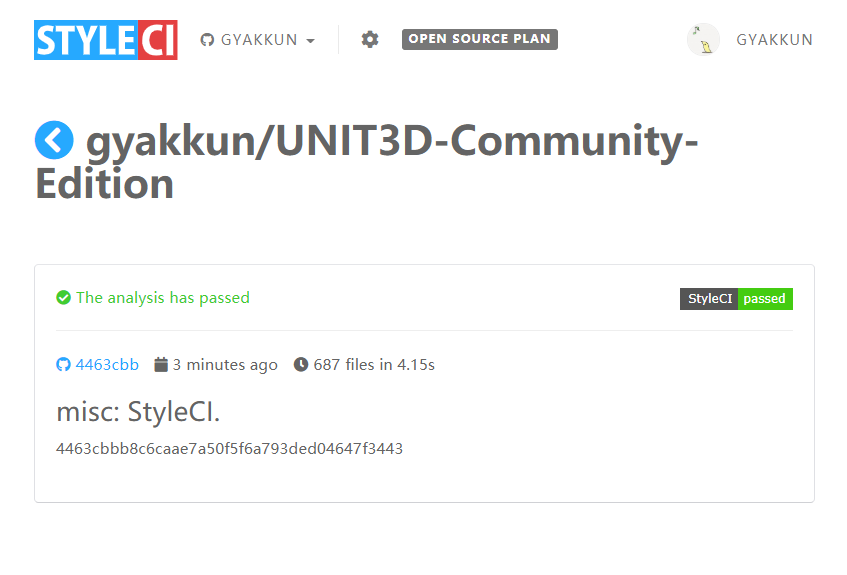
\includegraphics[width=\textwidth]{support-files/4.1-style-ci.png}
		\caption{StyleCI}
		\label{fig:styleci}
    \end{subfigure} \\
    \vbox{}
    % 全角空格占位, 否则空不出两行
     \\
    \vbox{}
	% \makebox[0.05\textwidth]{}
    \begin{subfigure}{0.8\textwidth}
		\centering
		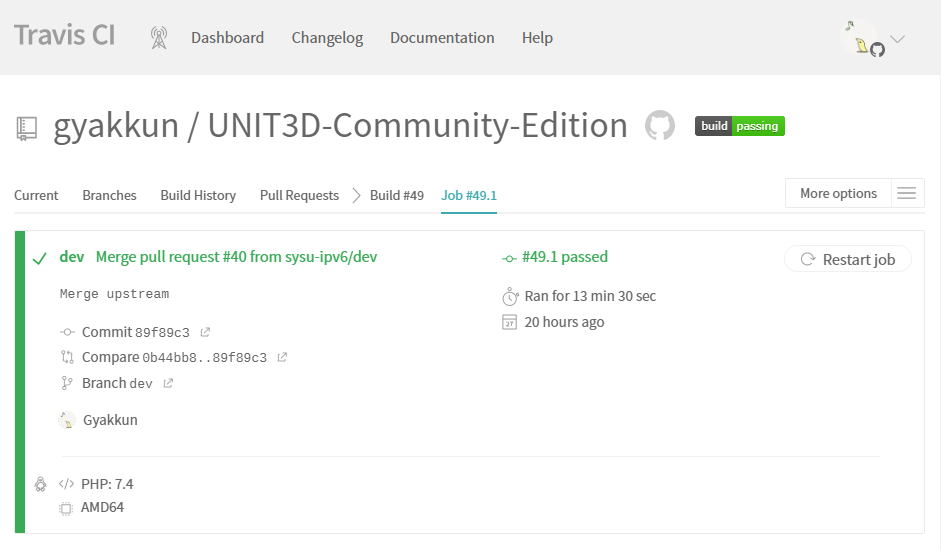
\includegraphics[width=\textwidth]{support-files/4.1-travis-ci.png}
		\caption{TravisCI}
		\label{fig:travisci}
	\end{subfigure} 
    % \makebox[0.05\textwidth]{}
    \caption{两种在线持续集成工具}
	\label{fig:ci}
\end{figure}

% [图 (4.1-style-ci, 4.1-travis-ci) TravisCI StyleCI]

具体的本地测试环境是在VMware虚拟机上, 通过PhpStorm的Deploy(部署)功能以及虚拟机的SSH(Secure Shell, 安全外壳协议)服务, 能够将代码实时地从本地开发环境同步到虚拟机的测试环境中。然后在本地开发环境的浏览器中就能实时预览到开发中的网页, 见图 \ref{fig:devenv}。

\begin{figure}[h]
	\centering
    \begin{subfigure}{0.8\textwidth}
		\centering
		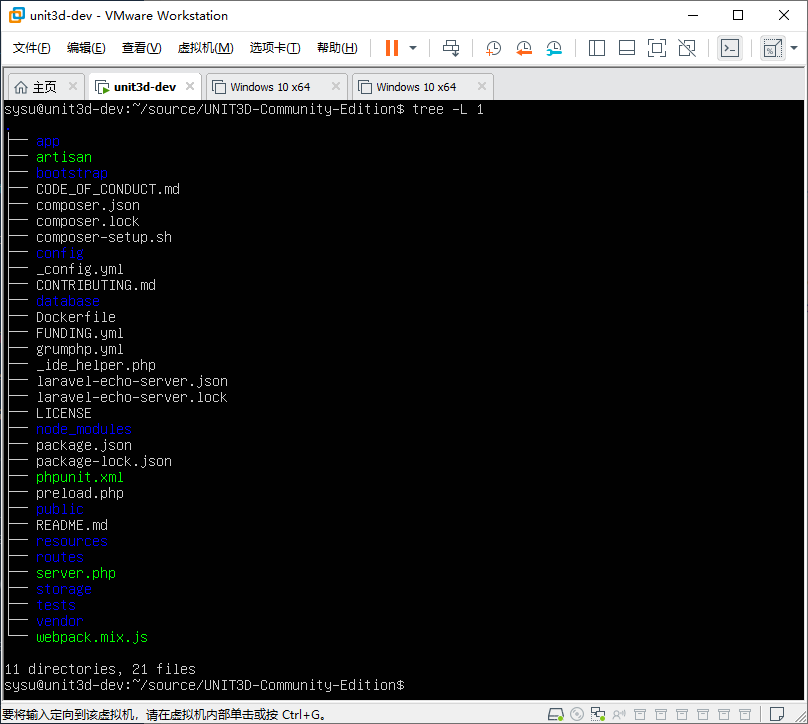
\includegraphics[width=\textwidth]{support-files/4.1-vwmare-unit3d-dev.png}
		\caption{VMware 下看到的目录结构}
		\label{fig:vmware}
	\end{subfigure} \\
    \vbox{}
    % 全角空格占位, 否则空不出两行
     \\
    \vbox{}
    \begin{subfigure}{0.8\textwidth}
		\centering
		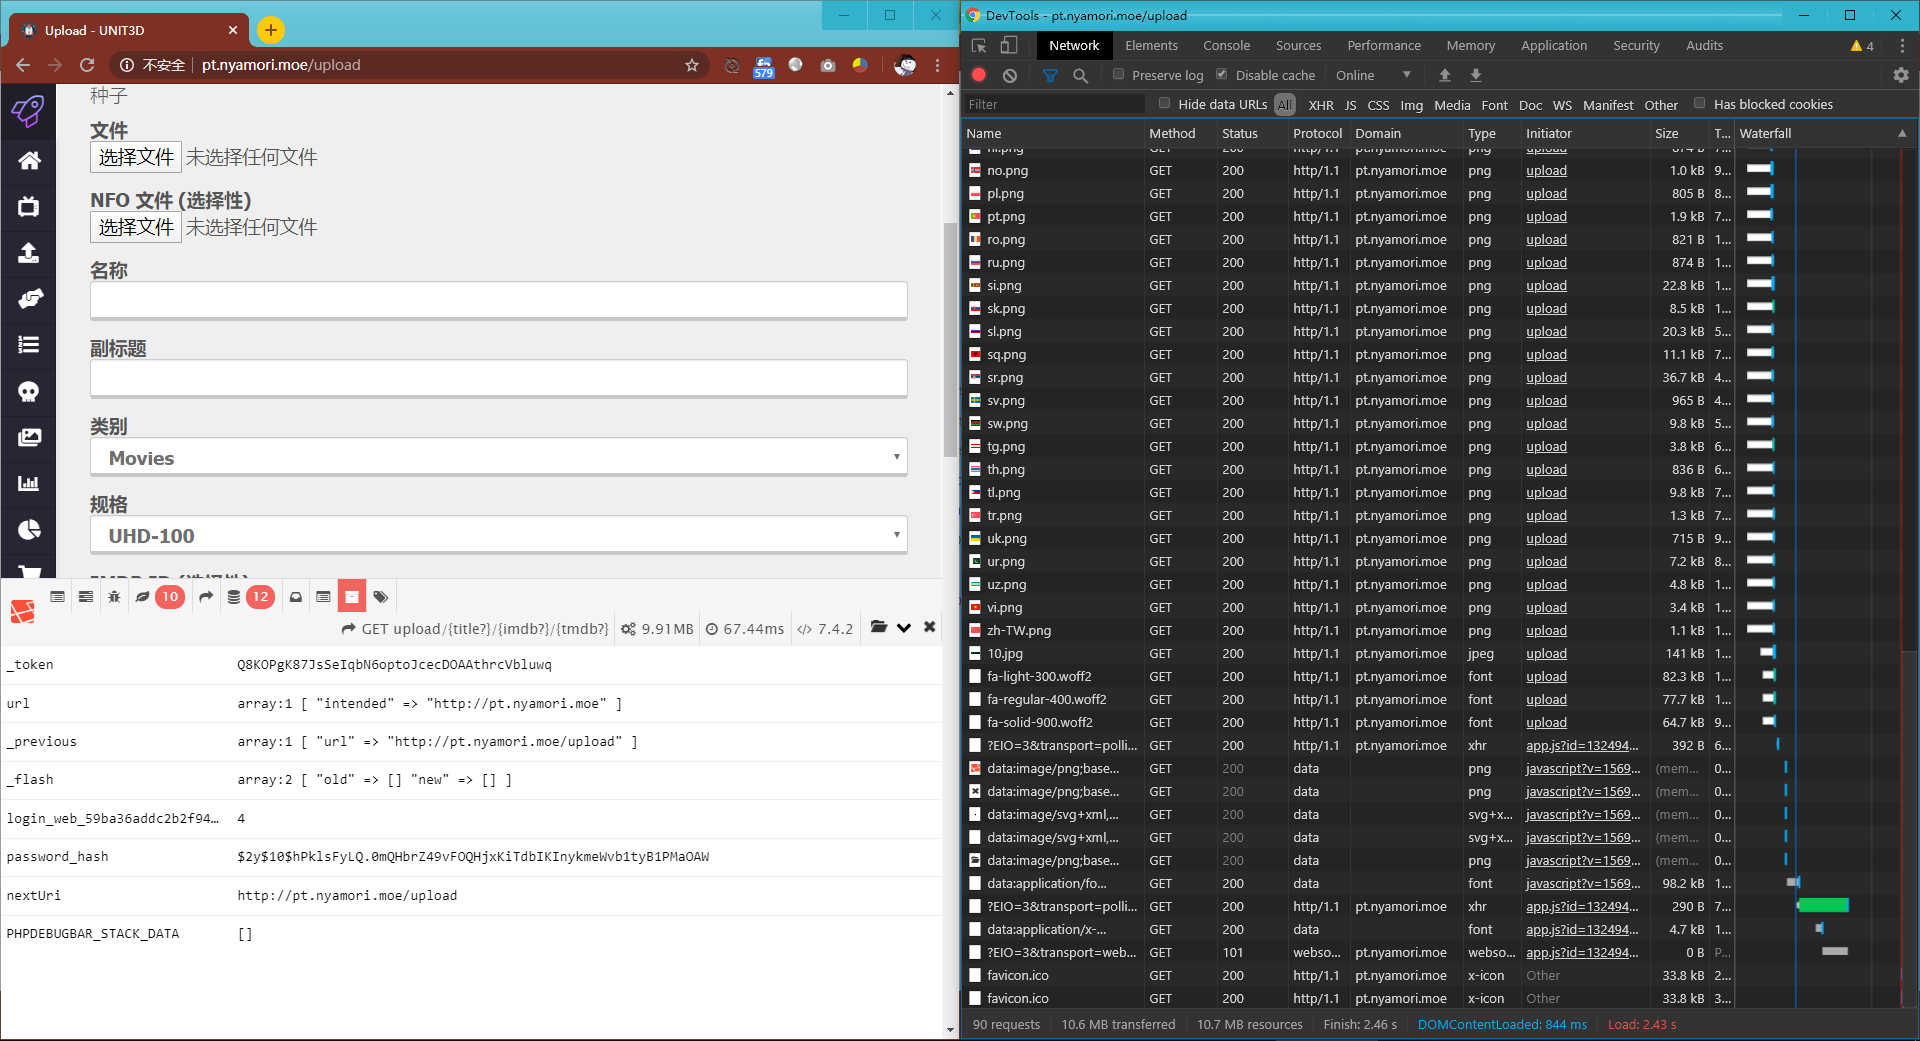
\includegraphics[width=\textwidth]{support-files/4.1-web-idehelper-chrome-devtool.png}
		\caption{调试中的网页}
		\label{fig:chromedevtool}
	\end{subfigure} 
    % \makebox[0.05\textwidth]{}
    \caption{调试环境}
	\label{fig:devenv}
\end{figure}

% [图 (4.1-vwmare-unit3d-dev, 4.1-web-idehelper-chrome-devtool) 虚拟机 和 调试阶段的页面 截图重点给到IDE HELPER 和网页下面的Dev Toolbar]

\section{本地化工作}

Laravel框架具有较好的国际化兼容性, 通过在资源文件中定义相应英文单词的特定语言翻译, 然后在视图模板文件中使用`@lang('app.langItem')'这种注记将原始内容表示出来, 就可以简单地通过前端的语言切换选项切换所渲染的不同语言界面。

\begin{figure}[ht]
    \centering
    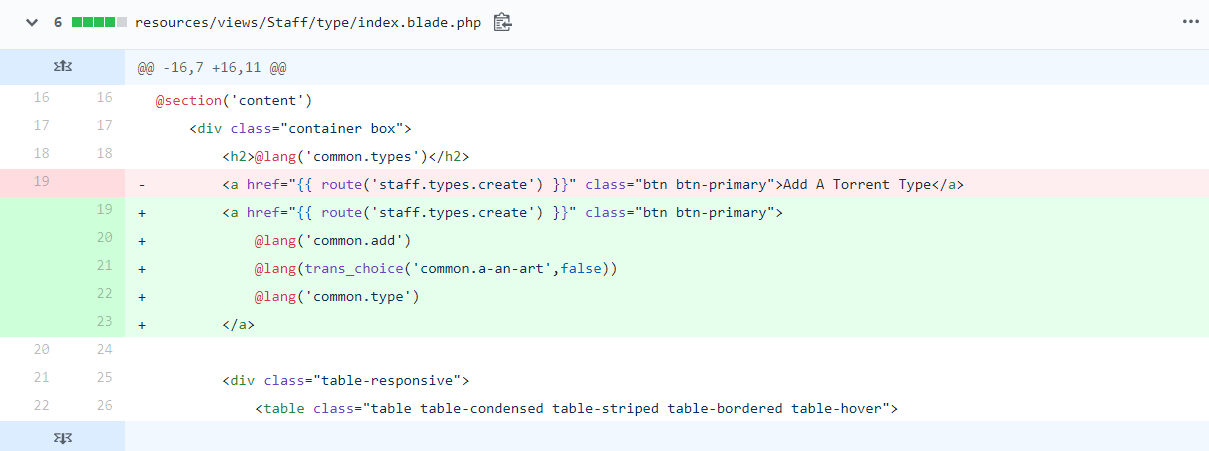
\includegraphics[width=0.9\textwidth]{support-files/4.2-git-diff.png}
    \caption{本地化所做的代码修改}
    \label{fig:localdiff}
\end{figure}

% [图 (4.2-git-diff) 一份git diff式的源码前后对比, 突出从原始英语单词到`@lang('app.langItem')'的部分]

针对英语转中文的翻译部分, 由于笔者曾经修过实用口译这门课程, 对快速高效的翻译颇有心得。经过一番重新翻译、修改、润色, 最终得到了令人满意的中文用户界面。

\begin{figure}[h]
	\centering
    \begin{subfigure}{0.3\textwidth}
        \centering
        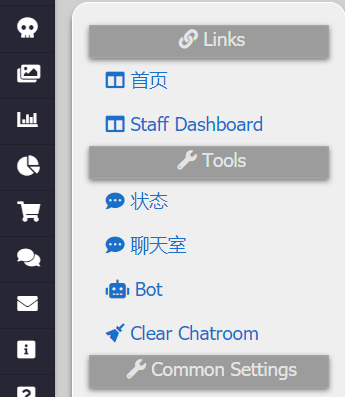
\includegraphics[width=\textwidth]{support-files/4.2-before-localization-cut.png}
        \caption{本地化前}
        \label{fig:beforelocal}
    \end{subfigure}
    \makebox[0.05\textwidth]{}
    \begin{subfigure}{0.3\textwidth}
        \centering
        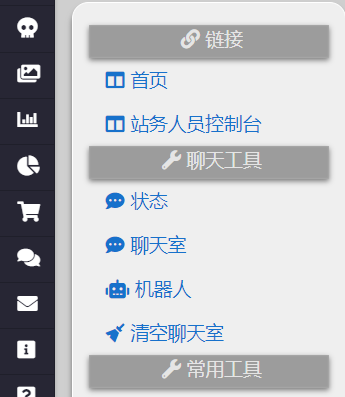
\includegraphics[width=\textwidth]{support-files/4.2-after-localization-cut.png}
        \caption{本地化后}
        \label{fig:afterlocal}
    \end{subfigure} \\
    % \makebox[0.05\textwidth]{}
    \caption{本地化前后的站务工作台页面对比}
    \label{fig:guidifflocal}
\end{figure}

% [图 (4.2-before-localization-cut, 4.2-after-localization-cut) 对比前后用户界面的语言部分]


\section{数据表迁移工作}
\label{sec:migration}

迁移脚本实际上就是将原表的字段一一对应到新表的字段中, 然后通过SQL语句逐条地重新录入。

前置步骤是将新表建立起来。这里用到了Laravel自带的`Illuminate\textbackslash Database\textbackslash Sche\-ma\textbackslash'类提供Migration子类。实际上, 所有数据库迁移操作基本都离不开对这个类类方法的使用。下图所示是给UNIT3D表结构中新增副标题(Subhead)字段的迁移脚本。

\begin{figure}[ht]
    \centering
    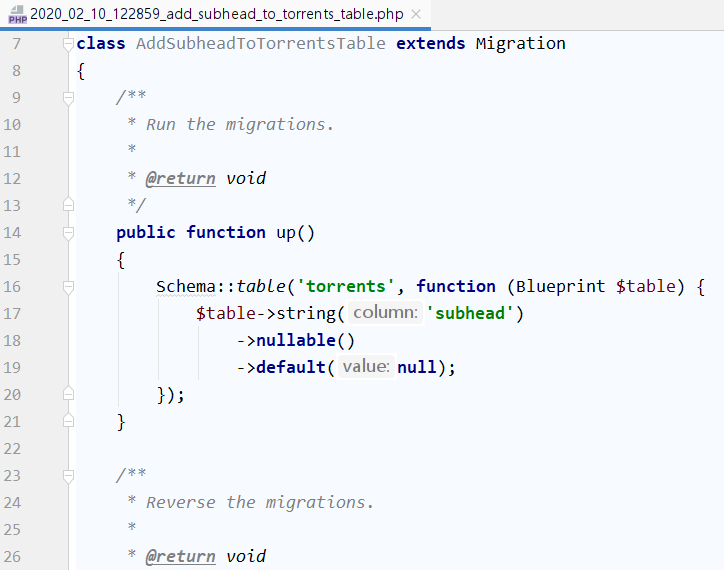
\includegraphics[width=0.9\textwidth]{support-files/4.3-subhead-migration-script.png}
    \caption{增加Subhead字段所用的迁移脚本}
    \label{fig:subheadmigratescript}
\end{figure}

% [图 (4.3-subhead-migration-script) 新表中新增subhead的脚本, 截图/database/migrations/2020\_02\_10\_122859\_add\_subhead\_to\_torrents\_table.php]

在这里, Blueprint类会将相应的Migration类方法, 比如`\$table->string('subhead')', 转化为SQL语句`alter table \$table add subhead', 从而达到增加字段的目的。

同时, Migration子类中定义了回溯的`down()'函数, 方便进行数据库迁移失败后的反向迁移。

具体的从NexusPHP迁移到UNIT3D的脚本, 包含了一个创建新表的脚本, 用到上述Blueprint类的子类方法, 按照目标的表结构创建数据表。还包含了一个描述新旧数据表各字段映射关系的`Mapping.php'文件, 里面的代码负责将旧表中的每一行数据解析, 转换成新表对应字段的`INSERT'SQL语句, 然后执行, 从而达到旧表迁移到新表的目的。

\begin{figure}[ht]
    \centering
    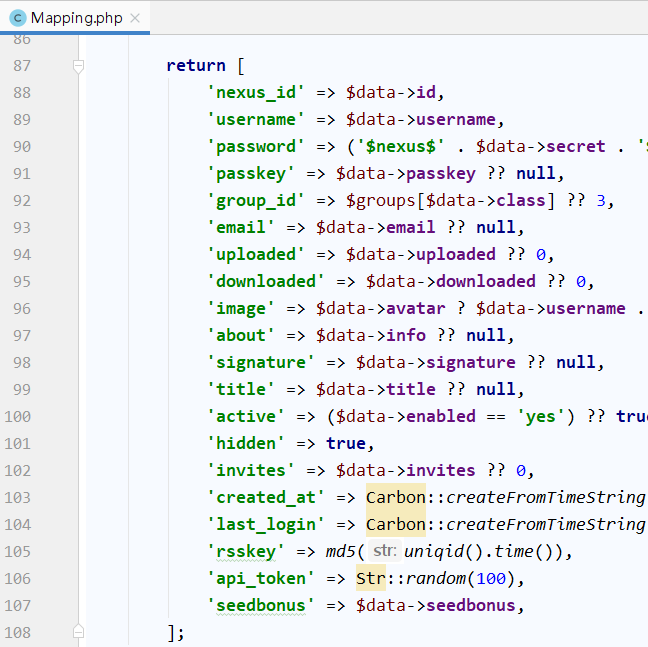
\includegraphics[width=0.6\textwidth]{support-files/4.3-tjupt-to-unit3d-script-mapping.png}
    \caption{新旧数据表的映射关系}
    \label{fig:mapnexusphpunit3d}
\end{figure}

% [图 (4.3-tjupt-to-unit3d-script-mapping) 旧表 vs 新表, 截取PHPSTORM中TJUPT\_TO\_UNIT3D中的Mapping.php]


\section{功能删改 - 标签功能调整}

事实上, \ref{subsec:tagadjust}中所描述的标签系统问题, 很大程度是因为UNIT3D数据表维护的种子元信息中, 有不少字段被设置为``必填项''。比如电影种子的`IMDB ID'项就属于对笔者一方非必要的字段, 但因为被设置为必填项, 故在测试阶段只能填无实际语义的样例值, 或者直接填0主动触发报错。该值又与标签系统向IMDB API的请求参数直接相关, 导致部署测试运行过程中的大量报错。

找到问题的原因之后, 笔者先尝试剔除诸如上述``电影''资源分类中`IMDB ID'字段的必要输入开关。其后, 因为在\ref{sec:migration}所描述的数据表迁移中, 为新表增加了很多其他资源类型项, 因此, 只要将自带的电影等分类从数据库中删除, 将新的分类设置成默认分类, 即可绕过上述标签的联网获取机制, 变相达到剔除标签功能的目的。

\begin{figure}[ht]
    \centering
    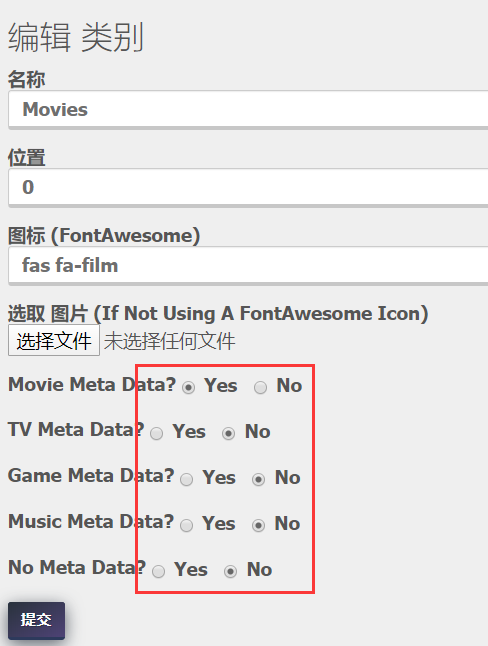
\includegraphics[width=0.45\textwidth]{support-files/4.4-remove-requirement-for-tag-system.png}
    \caption{取消必要字段开关}
    \label{fig:disableforcemeta}
\end{figure}

\section{功能增添 - 投票功能的实现}

投票功能可以用在统计信息, 收集用户意见, 交由用户对网站内外的大事小情进行表态, 从而决定网站的运营、开发方向, 是实用性相当高的一个功能。该功能未能具体完整地实现, 不得不说是UNIT3D原版的一大缺憾。

UNIT3D的数据库中定义有poll和voters两个数据表。乍一看很容易混淆, 实际上poll里的项代表被发起的一次投票, voters的项则代表每人次投出去的票, 记录着投票人、投票选项以及投票时发起的HTTP请求的源IP地址。同时, 为了记录投票的选项, 还使用一张option表来存储每个投票的选项。

UNIT3D原版实现了增加单项投票的功能。然而, 删/改投票, 多选投票, 以及投票的重复IP检查功能都尚处于桩函数的状态, 相关的网页前端只留了一个`\#'的空锚点, 并无有效超链接路径。为此, 笔者对投票的删除、修改, 多选投票, 以及投票的重复IP检查进行了具体的实现。

\subsection{投票的删除、修改}

投票的增删改主要涉及到`/app/Http/Controllers/Staff/PollControler.php'这个控制器以及`/resources/views/Staff/poll/'下的相应视图模板。

对于控制器, 笔者增加了`update(\$id)', `destroy(\$id)'函数。其中`update(\$id)'函数包含了对既有投票的修改。`destroy(\$id)'则根据投票的唯一ID在数据库中删除相应的投票。

在修改投票的过程中, 管理员可能增加/删除/修改既有的选项名称。为此, 需要从前端请求中获取相应的选项ID, 然后比对数据表中相应ID的既有选项名称是否和前端返回的选项名称一致, 若不一致, 则将其加入临时待增加/修改/删除选项数组中, 在之后的循环中逐一从数据库中增加/修改/删除。流程图见图 \ref{fig:updateflowchart}。

这里用到了不少前端的技巧。为了使前端的修改请求能够带上原始选项的ID, 笔者在控制器返回给前端的修改投票页面里的具体各个投票的区块中, 增加了非显示字段`poll-id'以及`option-id', 顾名思义, 就是数据表中对应投票/选项的唯一ID。在前端将要提交的表单中, 这两项会一并提交, 从而在后端的控制器中能取到相应的ID, 继而进入上述`update(\$id)'函数的流程中。

\begin{figure}[h]
    \centering
    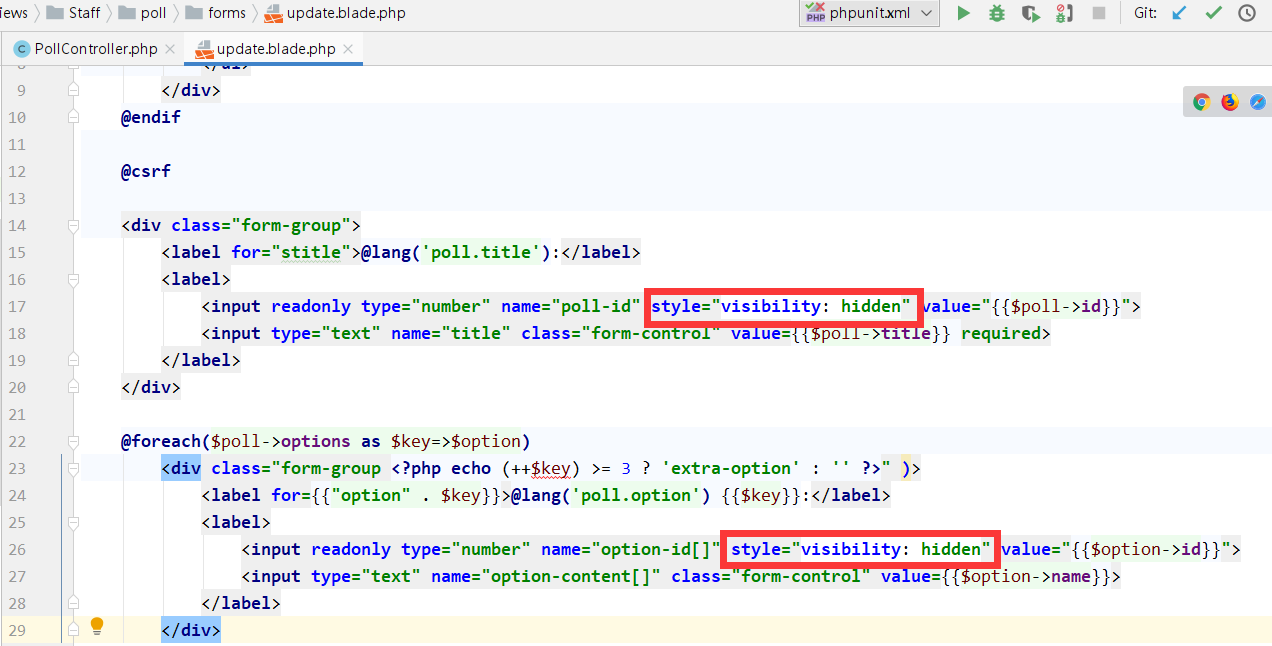
\includegraphics[width=0.8\textwidth]{support-files/4.5.1-visibility-hidden.png}
    \caption{在模板中设置visibility:hidden}
    \label{fig:visibilityhidden}
\end{figure}

删除的逻辑类似, 从前端取得待删除的投票ID后, 交由Laravel的模型模块, 自动注入相关类方法, 继而从数据表中实际删除对应的投票。

\begin{figure}[hbp]
    \centering
    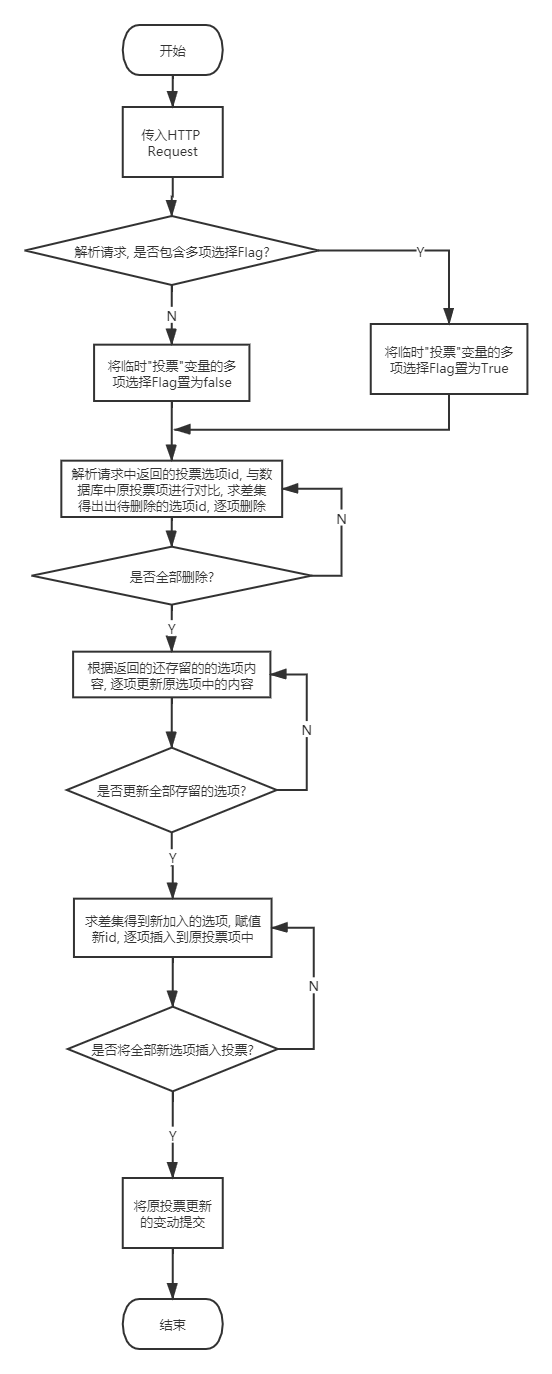
\includegraphics[width=0.37\textwidth]{support-files/4.5.1-pollcontroller-update-flowchart.png}
    \caption{update()函数的流程图}
    \label{fig:updateflowchart}
\end{figure}

\newpage

\subsection{投票的重复IP校验}

重复IP校验的逻辑并不复杂, 只要将每次投票的HTTP请求中的源IP提取出来, 再与voter数据表中相应poll\_id外键对应的所有票的ip字段进行比对, 若发现一致的, 则判定为重复IP。

\begin{figure}[hb]
    \centering
    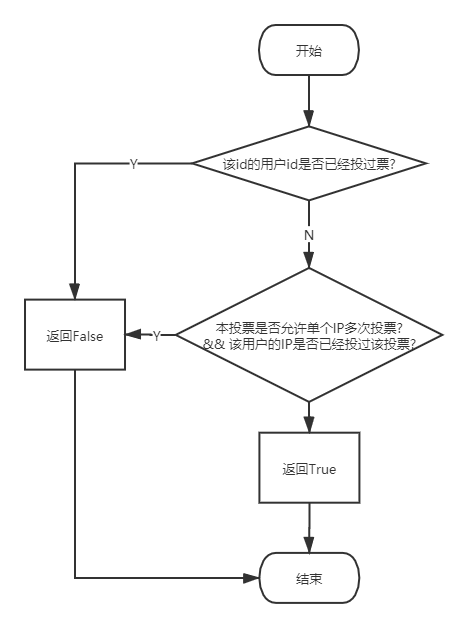
\includegraphics[width=0.2\textwidth]{support-files/4.5.2-validate-voter-flowchart.png}
    \caption{validateVoter()函数的流程图}
    \label{fig:validatevoterchart}
\end{figure}

% [图 (4.5.2-validate-voter-flowchart) 判定重复IP流程图 app\textbackslash Http\textbackslash Controllers\textbackslash PollController.php  validateVoter()函数]

具体的实现中, 使用了或非运算符简化运算, 但语义不太明晰。

\begin{figure}[h]
    \centering
    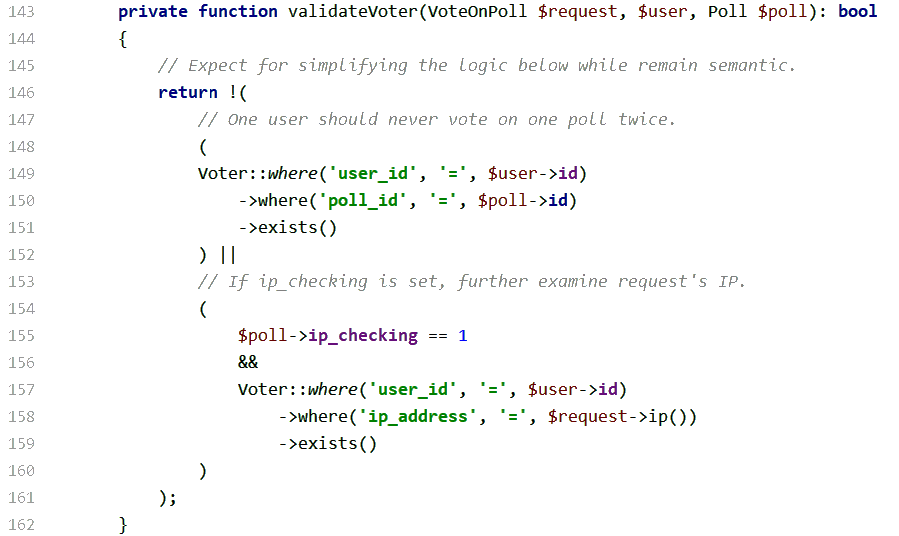
\includegraphics[width=0.8\textwidth]{support-files/4.5.2-validate-voter-code.png}
    \caption{validateVoter()函数的具体代码}
    \label{fig:validatevotercode}
\end{figure}

% [图  (4.5.2-validate-voter-code) 直接糊代码 app\textbackslash Http\textbackslash Controllers\textbackslash PollController.php  validateVoter()函数]


\section{功能增添 - 初步添加鉴权操作日志记录功能}

由于\ref{subsec:auth}中描述的理由, 需要为系统添加鉴权操作日志功能(以下记作``鉴权日志'')。鉴权日志需要定义一个全新的数据模型, 并对应一张新的数据表, 因此需要进行一定的上层设计及数据库的迁移。

\subsection{数据模型的定义}

因为主要记录的是鉴权操作, 而HTTP服务器软件, 比如nginx\footnote{\url{https://www.nginx.com/}}, 都有独自完善的日志功能, 所以本平台的鉴权日志只需记录用户相关的信息, 以及根据用户所用的设备等具有辨识性质信息哈希得到的一个识别码。为此, 定义Authentication类, 记录'user\_id', 'device\_id','ip\_address'三个字段, 分别对应PHP的integer, integer和string原生类型。为了记录鉴权的状态, 定义三种字符串常量, 'LOGIN', 'FAILED', 'LOCKOUT', 分别表示登录(即鉴权成功), 失败(表示当此鉴权操作失败, 如密码错误), 以及锁定(账户多次鉴权操作失败, 账户被上锁, 待解封) 之后的持久化步骤交给Laravel的持久化模块。

\begin{figure}[h]
    \centering
    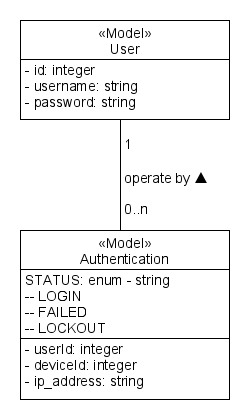
\includegraphics[width=0.45\textwidth]{support-files/4.6.1-authentication-model-png.png}
    \caption{User类和Authentication类的E-R图}
    \label{fig:userauthmodeler}
\end{figure}

% [图 (4.6.1-authentication-model-png) models/authentication.php 可以用UML画E-R图]


\subsection{数据库迁移脚本}

为了记录前述的数据模型, 要在数据库中定义新的数据表。这里用到前述的数据库迁移脚本。只需要将新字段的名称和SQL数据类型通过Blueprint类的相应子类类方法告知数据库即可。

\begin{figure}[h]
    \centering
    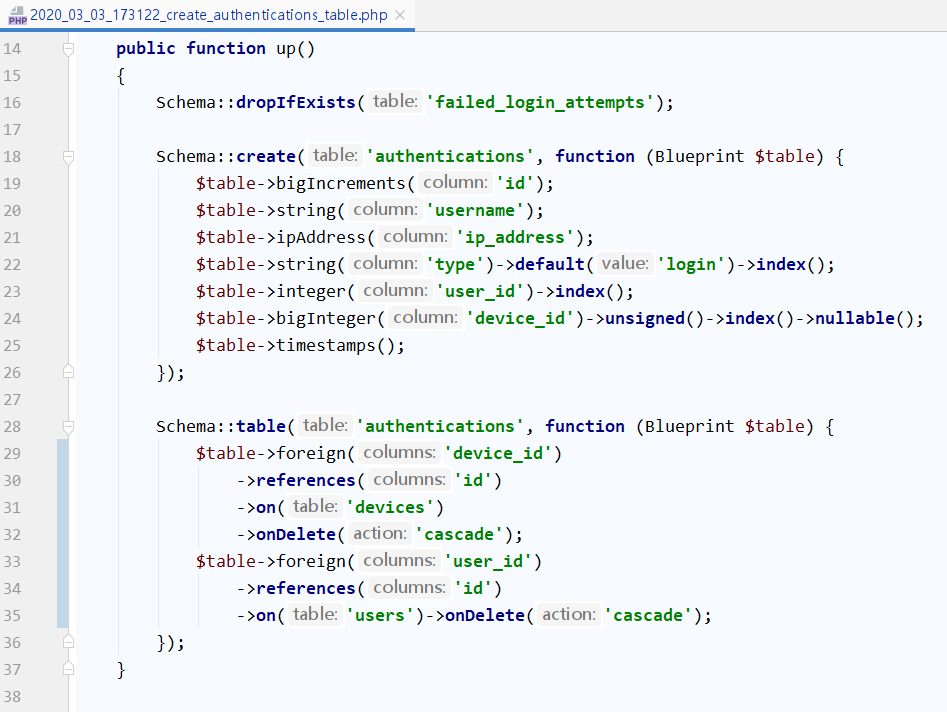
\includegraphics[width=0.8\textwidth]{support-files/4.6.1-migration-script.png}
    \caption{针对Authentication表的数据库迁移脚本}
    \label{fig:authmigratescript}
\end{figure}

% [图 (4.6.1-migration-script) \textbackslash database\textbackslash migrations\textbackslash 2020\_03\_03\_173122\_create\_authentications\_table.php]

\subsection{具体的日志记录逻辑}

为了实现日志记录, 需要为每一次鉴权操作注册监听事件。为此需要在Laravel框架中的事件监听服务中注册鉴权操作的事件订阅者(AuthEventSubscriber), 流程图如下。

% [图 (4.6.3-event-model) 摘要Laravel的事件监听机制]


\section{网站的上线部署}

网站的上线主要是站长17级软件工程专业的howardlau同学在负责。具体的上线方式是采用Docker部署, MySQL数据库和Redis缓存服务也使用既有的Docker镜像, 通过``docker-compose''\footnote{\url{https://docs.docker.com/compose}}将其组合成容器, 方便今后交付到诸如Kubernete等的容器化云平台上投入生产使用。

\section{试运行}
\label{sec:preop}

笔者及同好通过SYSU IPv6交流群\footnote{一个群员以中山大学数据科学与计算机学院学生为主的兴趣交流QQ群}以及相关公众号推送\footnote{微信公众号: SYSPT}招募内测用户。用户群体主要是数据科学与计算机学院的学生, 他们对BT协议以及PT网站都有一定的了解, 有些还是北邮人BYRBT和六维空间的忠实用户。对于这样内测用户, 不用重新培养使用习惯, 能够较好地帮助运营方确定用户需求, 并得以迅速跟进开发实现。

而对另一部分通过推送慕名而来的BT新手, 笔者及同好还有数据科学与计算机学院的热心同学们热情地为他们提供了帮助。通过这样良好的内部交流, 循环促进培养新人的用户习惯, 整个网站的建设正在有条不紊地推进中。
